\section{Key Results}

\begin{frame}
\frametitle{Community Structure: Heterogeneous Organization}

\begin{table}[ht]
\centering
\begin{tabular}{|c|c|c|}
\hline
\textbf{Community} & \textbf{Investors} & \textbf{Investment Share} \\
\hline
0 & 4,248 & 19.4\% \\
1 & 4,089 & 10.4\% \\
2 & 3,959 & \textbf{33.6\%} \\
Cross-community & --- & 35.1\% \\
\hline
\end{tabular}
\caption{Distribution of co-investment activity}
\end{table}

\begin{itemize}
    \item \textbf{Community 2}: Despite similar size, handles 75\% more investments than Community 0
    \item Substantial cross-community collaboration (35.1\%)
    \item Suggests structural differences drive efficiency
\end{itemize}

\end{frame}

\begin{frame}
\frametitle{Geographic Clustering: Silicon Valley Dominance}

\begin{figure}
    \centering
    
\includegraphics[width=0.6\textwidth]{../figures/us/categorical_comparison_investor_region_right.png}
    % \caption{Geographic distribution - Early-stage investors}
\end{figure}

\vspace{-0.5cm}
\begin{itemize}
    \item \textbf{Community 2}: Exceptional Silicon Valley concentration
    \item \textbf{Community 1}: More internationally diversified
    \item \textbf{Community 0}: Balanced U.S. distribution
\end{itemize}

\end{frame}

\begin{frame}
\frametitle{Network Structure: Power-Law Patterns}

\begin{figure}
    \centering
    
\includegraphics[width=\textwidth]{../figures/us/node_degree_distributions_comprehensive_pt1.png}
    % \caption{Degree distributions across communities}
\end{figure}

\begin{itemize}
    \item All communities exhibit heavy-tailed, scale-free patterns
    \item Community 2 shows highest connectivity across all degree ranges
    \item Hub investors in Community 2 concentrated in early-stage (SV Angel, A16z, Khosla)
\end{itemize}

\end{frame}

\begin{frame}
\frametitle{Main Finding: Significant Nestedness in Silicon Valley}

\begin{figure}
    \centering
    
\includegraphics[width=0.75\textwidth]{../figures/us/nestedness_by_community_size.png}
    \caption{Nestedness vs. community size. Tests reveal only Silicon Valley community exhibits statistically high nestedness}
\end{figure}

\begin{alertblock}{Key Discovery}
\textbf{Only Silicon Valley community} exhibits statistically significant nestedness - hierarchical organization where specialists partner with subsets of generalists' connections.
\end{alertblock}

\end{frame}

\begin{frame}
\frametitle{Nestedness Visualization}

\begin{figure}
    \centering
    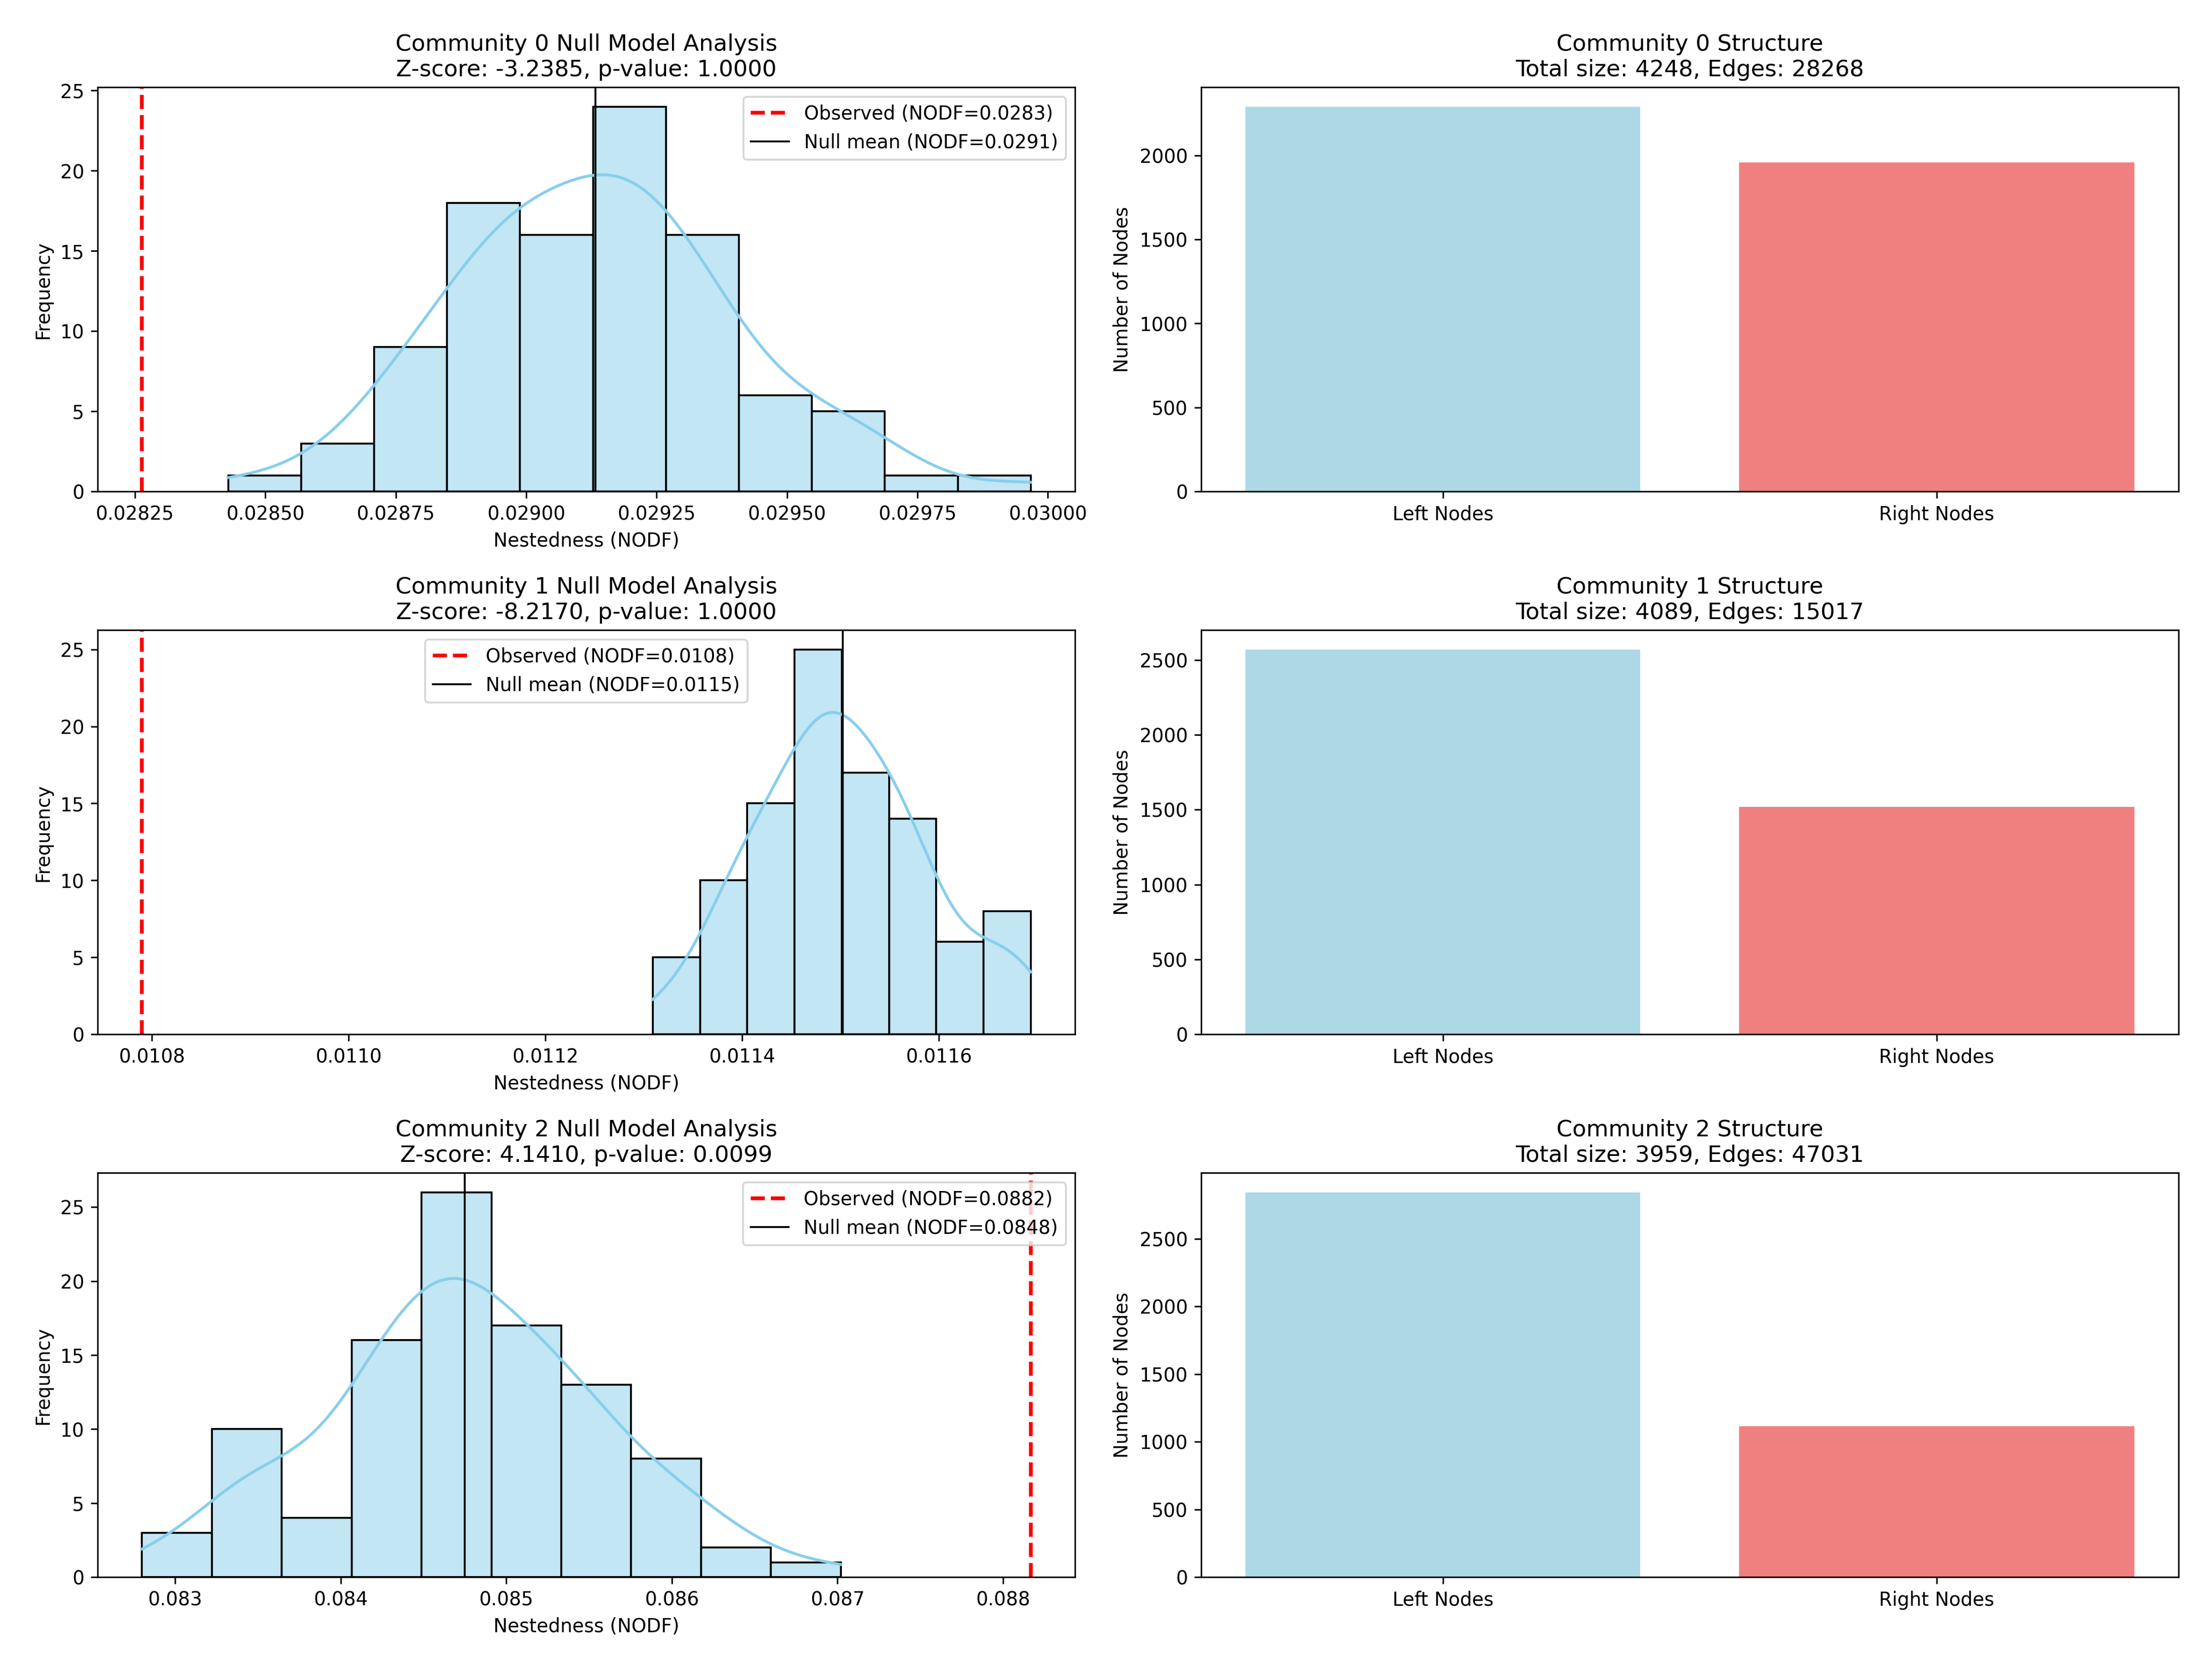
\includegraphics[width=0.8\textwidth]{../figures/mod/significant_communities_detailed_v2.png}
    \caption{Observed vs. null model nestedness distributions}
\end{figure}

% \begin{itemize}
%     \item Red line = observed nestedness
%     \item Blue distribution = random expectation
%     \item Only Community 2 significantly exceeds random baseline
% \end{itemize}

\end{frame}

\begin{frame}
\frametitle{Temporal Evolution: Progressive Development}

\begin{figure}
    \centering
    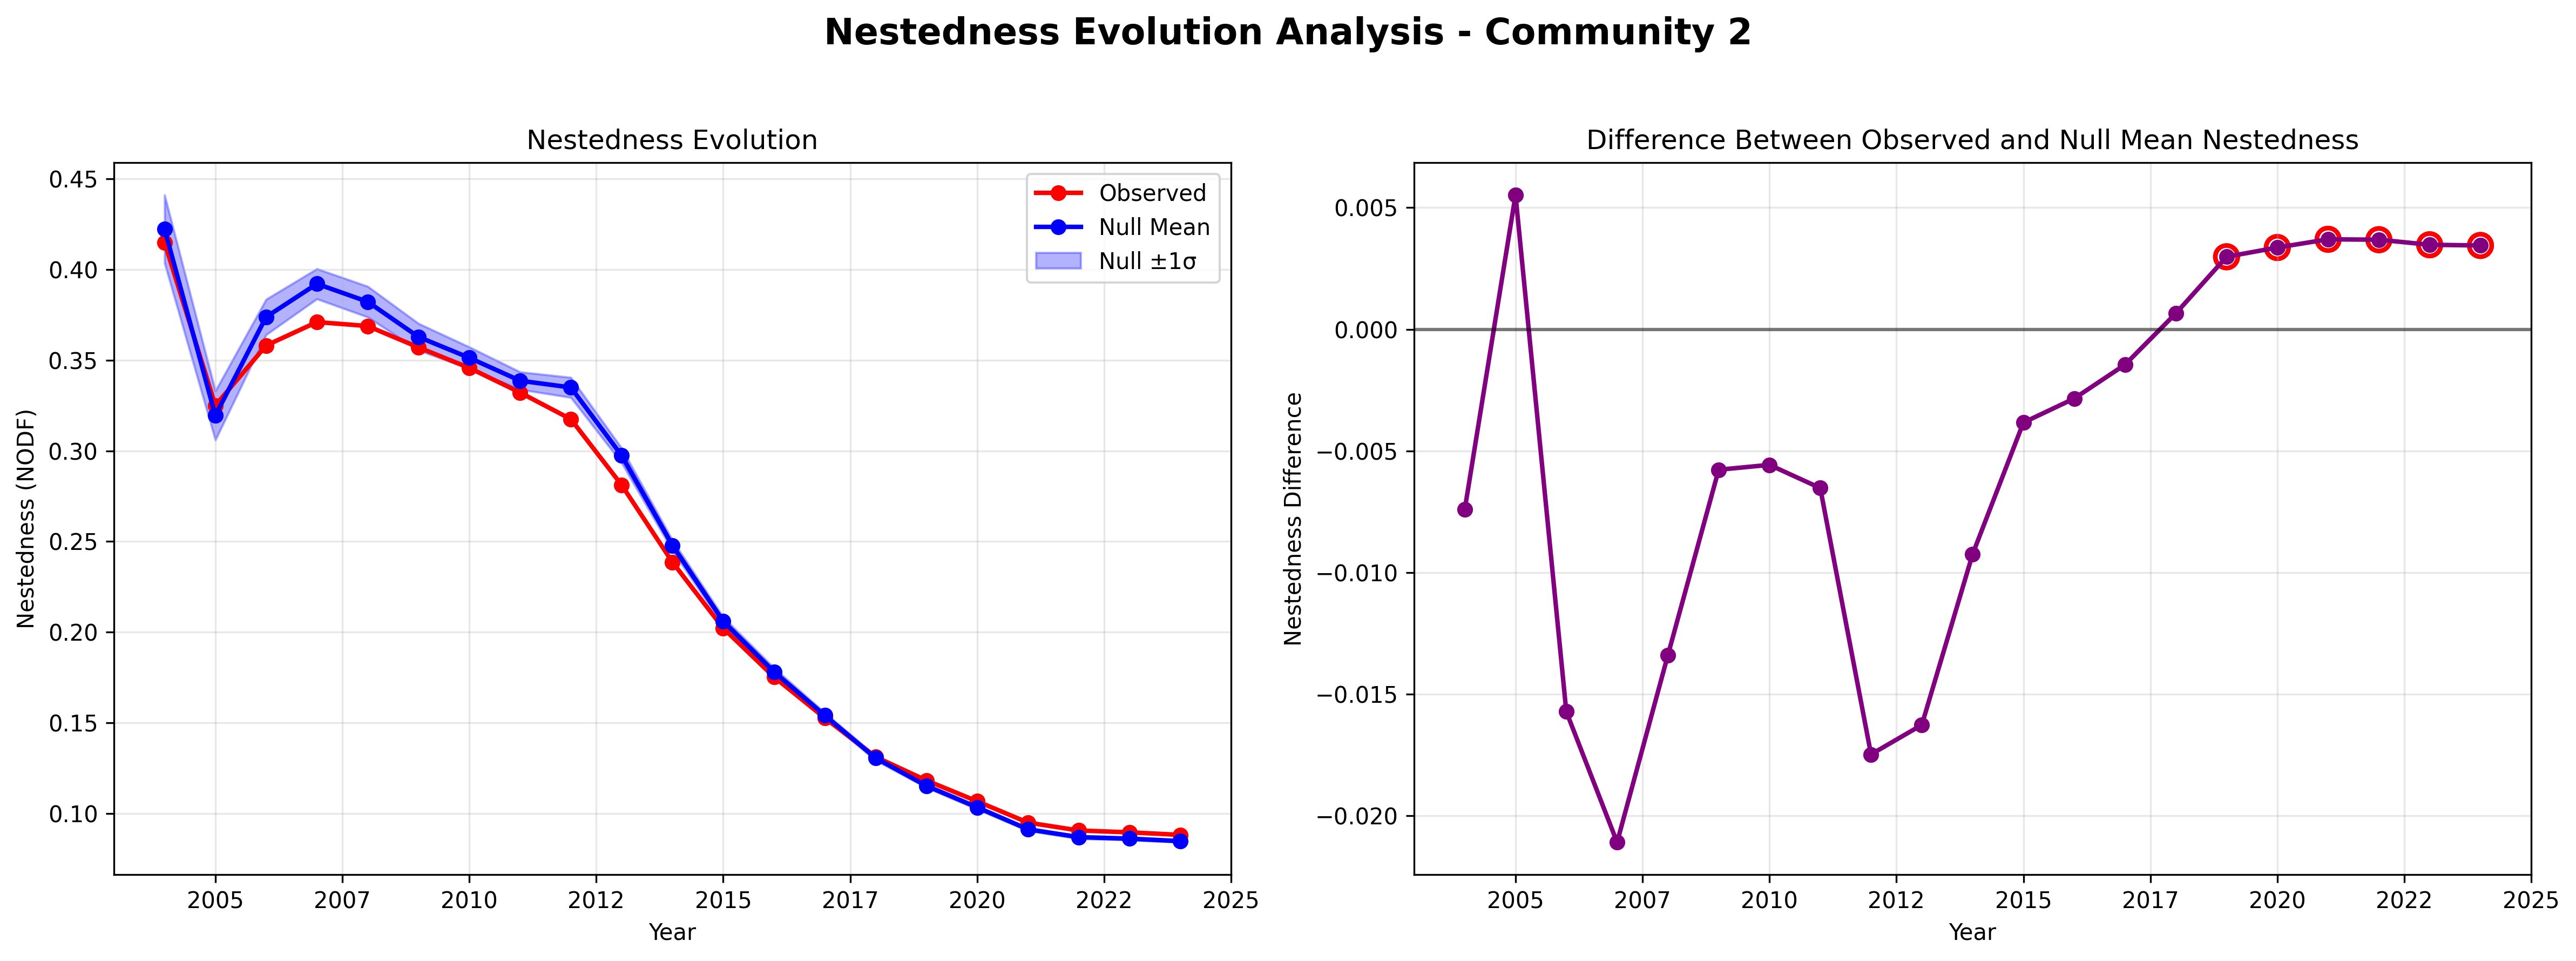
\includegraphics[width=\textwidth]{../figures/us/nestedness_evolution_community_2_pt1.png}
    % \caption{Nestedness evolution in Silicon Valley community (2007-2024)}
\end{figure}

\begin{itemize}
    \item \textbf{2007-2018}: Significantly low nestedness
    \item \textbf{2012+}: Gradual increase begins
    \item \textbf{2019}: Statistical significance achieved
    \item \textbf{2019-2024}: Sustained high nestedness
\end{itemize}

\end{frame}

\begin{frame}
\frametitle{Three-Phase Evolution Pattern}

\begin{figure}
    \centering
    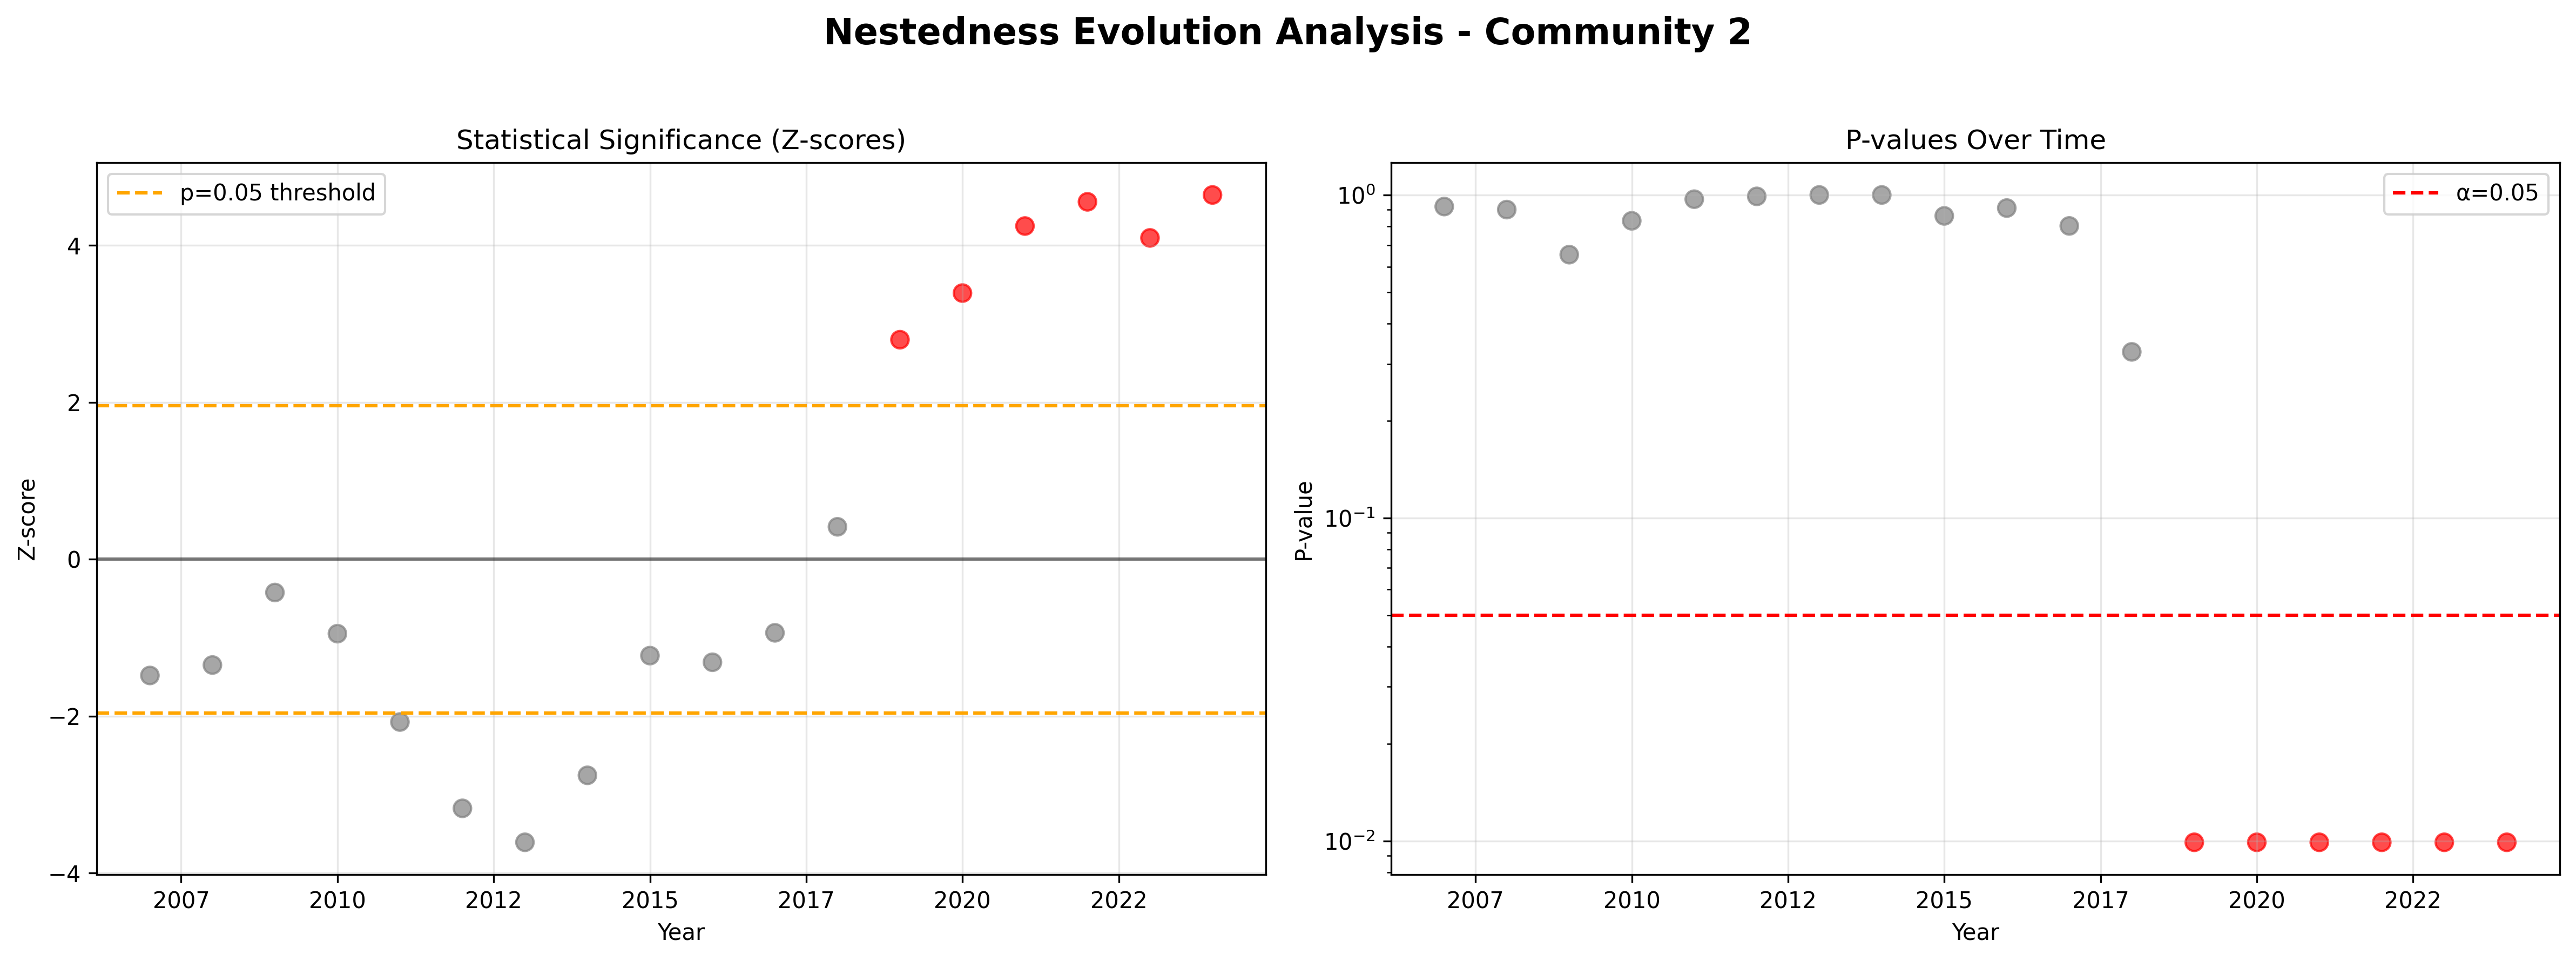
\includegraphics[width=\textwidth]{../figures/us/nestedness_evolution_community_2_pt2.png}
    \caption{Connectance evolution and significance achievement}
\end{figure}
\vspace{-0.4cm}
\begin{block}{Interpretation}
Nestedness develops \textbf{progressively} rather than suddenly - hierarchical organization accumulates over time before crossing significance thresholds.
\end{block}

\end{frame}

\begin{frame}
\frametitle{Network Growth and Structural Change}

\begin{figure}
    \centering
    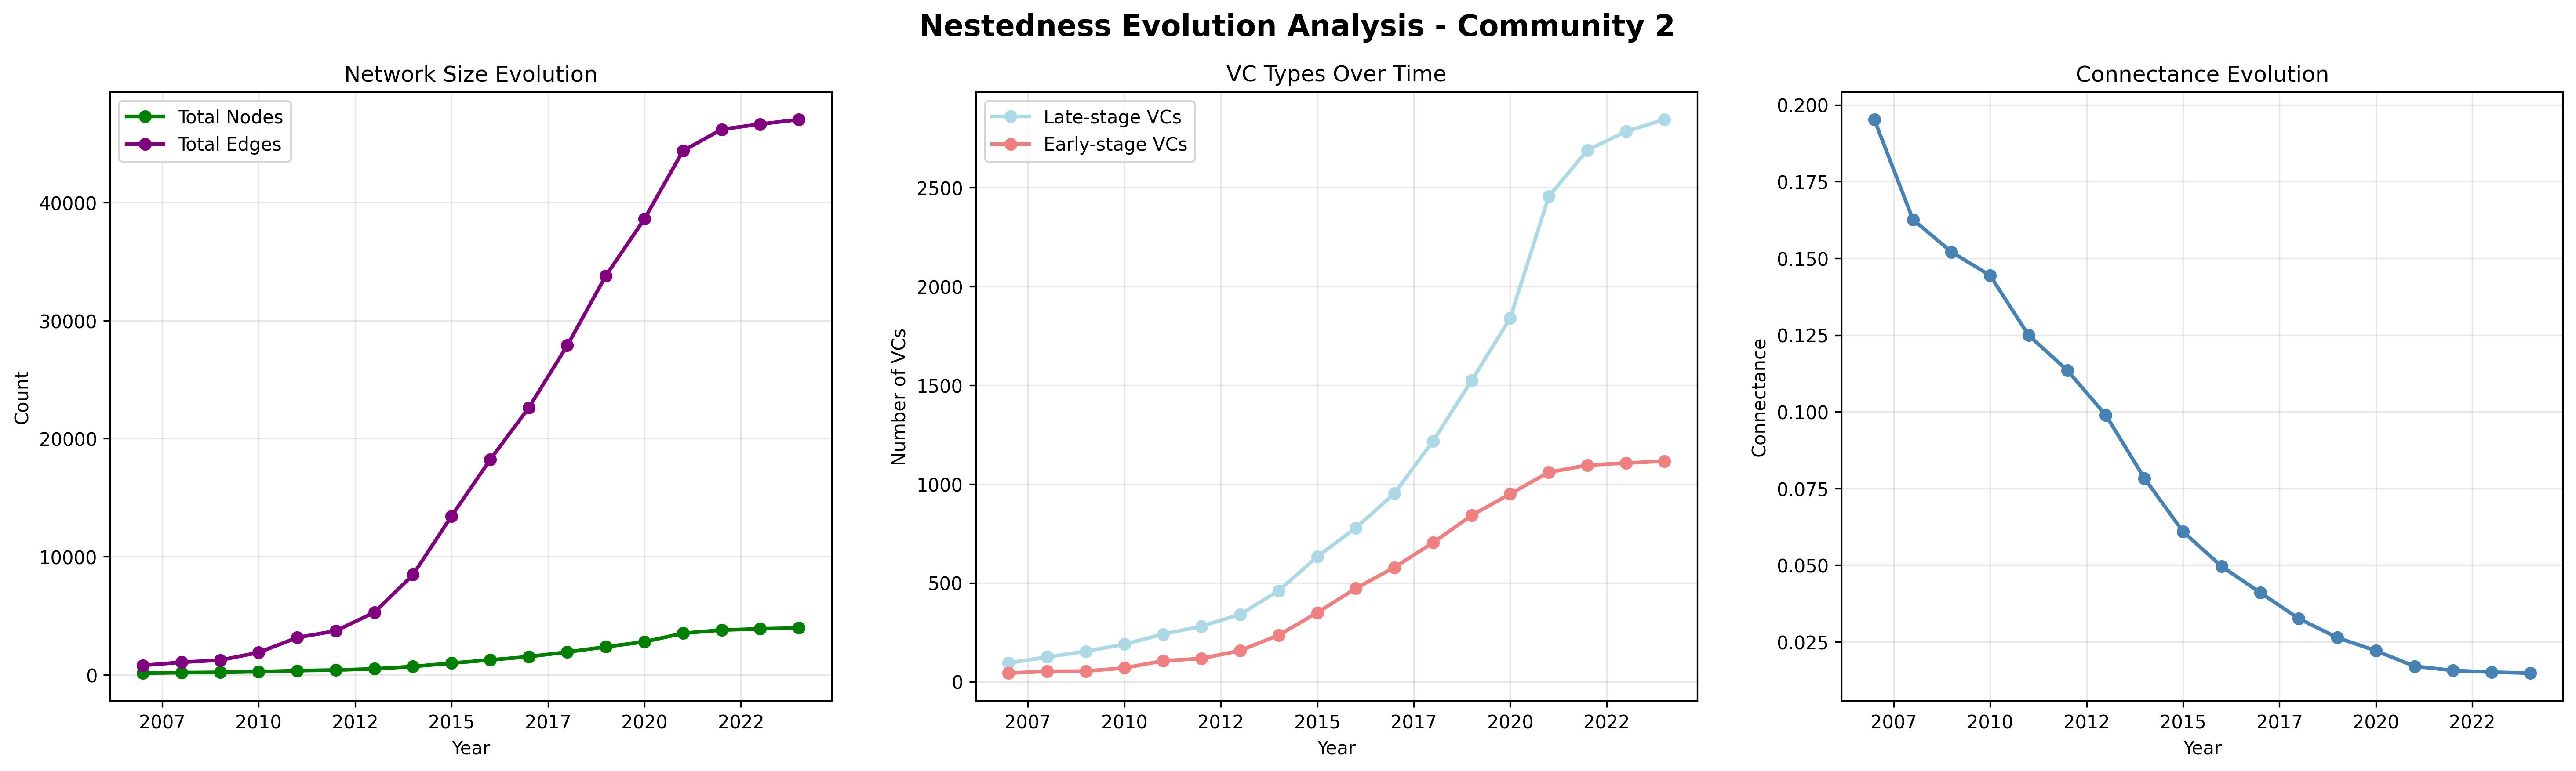
\includegraphics[width=\textwidth]{../figures/us/nestedness_evolution_community_2_pt3.png}
    \caption{Connectance evolution and significance achievement}
\end{figure}

\begin{itemize}
    \item Network becomes \textbf{sparser} (decreasing connectance) yet more \textbf{hierarchically organized}
    \item Critical threshold around 0.026 connectance
    \item Lower absolute nestedness but higher statistical significance over time
\end{itemize}

\end{frame}
